\hypertarget{lecture-13-notes}{%
\section{Lecture 13 Notes}\label{lecture-13-notes}}

\hypertarget{professor-prof.-lalitha-vadlamani}{%
\subsection{Professor : Prof.~Lalitha
Vadlamani}\label{professor-prof.-lalitha-vadlamani}}

\hypertarget{authors-ananya-sane-l-lakshmanan}{%
\subsection{Authors : Ananya Sane, L
Lakshmanan}\label{authors-ananya-sane-l-lakshmanan}}

\begin{center}\rule{0.5\linewidth}{0.5pt}\end{center}

\hypertarget{key-ideas}{%
\subsection{Key Ideas}\label{key-ideas}}

\begin{enumerate}
\def\labelenumi{\arabic{enumi}.}
\tightlist
\item
  Variance
\item
  Examples and Properties of Discrete Random Variables
\item
  Examples and Properties of Continuous Random Variables
\end{enumerate}

\begin{center}\rule{0.5\linewidth}{0.5pt}\end{center}

\hypertarget{variance-of-a-random-variable}{%
\subsection{Variance of a Random
Variable}\label{variance-of-a-random-variable}}

Variance can be understood as a quantity that represents the avergae
variation of a R.V about the mean. Given a R.V X, its variance is given
by

\(Var(X) = E[(X - E(X))^2] = E(X^2) - (E(X))^2\)

If X is discrete, then

\(E(X) = \mu\)

\(Var(X) = \displaystyle\sum_{x_i}(x_i-\mu)^2P_X(x_i)\)

If X is continuous, then

\(E(X) = \mu\)

\(Var(X) = \displaystyle\int_{-\infty}^{\infty}(x-\mu)^2f_X(x)dx\)

\hypertarget{properties-of-variance}{%
\subsubsection{Properties of Variance}\label{properties-of-variance}}

Variance is always \(\geq0\), with equality iff the random variable is
constant.

\begin{center}\rule{0.5\linewidth}{0.5pt}\end{center}

\hypertarget{examples-of-discrete-random-variables}{%
\subsection{Examples of Discrete Random
Variables}\label{examples-of-discrete-random-variables}}

\hypertarget{bernoulli-random-variables}{%
\subsubsection{1. Bernoulli Random
Variables}\label{bernoulli-random-variables}}

\begin{itemize}
\item
  Defined by

  \(P_X(x) = \begin{cases}p & for \ x=1\\1-p & for\ x=0\\0 & otherwise\end{cases}\)

  where \(0 < p < 1\).
\item
  \(E(X) = 0(1-p) + 1(p) = p\)
\item
  \(Var(X) = (0-p)^2(1-p) + (1-p)^2(p) = p(1-p)\)

  \begin{figure}
  \centering
  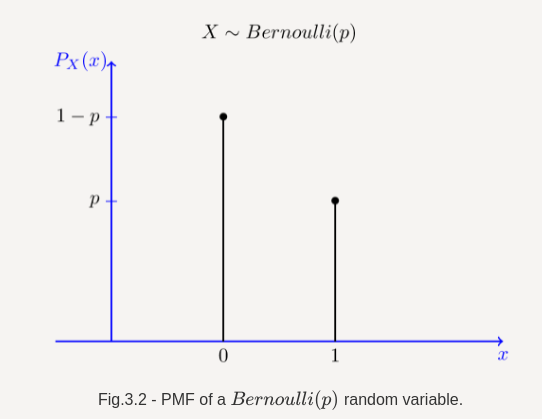
\includegraphics{Lecture 13 Notes e842fef9a3e0449fa78bac59b75dbc5c/Screenshot_from_2021-08-06_23-12-43.png}
  \caption{PMF of a Bernoulli random variable}
  \end{figure}
\item
  This random variable is mainly used to model random experiments that
  have two possible outcomes, which are sometimes referred to as
  ``success'' and ``failure''.
\item
  The Bernoulli random variable is also called the \textbf{Indicator
  random variable}, which tells us if a particular event has occured or
  not.
\end{itemize}

\hypertarget{binomial-random-variables}{%
\subsubsection{2. Binomial Random
Variables}\label{binomial-random-variables}}

\begin{itemize}
\item
  Experiment: Biased coin tossed \(n\) times with probability of heads
  being \(p\); outcomes mapped to \(k\) where \(k\) is the number of
  heads obtained.
\item
  This variable can be represented as the sum of \(n\) independent
  Bernoulli R.Vs.
\item
  \(E(X) = \displaystyle\sum_{i=0}^{n}i{n \choose i}p^i(1-p)^{n-i} = np\)
\item
  \(Var(X) =\) Sum of variances of \(n\) Bernoulli variables
  \(=nVar(X) = np(1-p)\)

  \begin{figure}
  \centering
  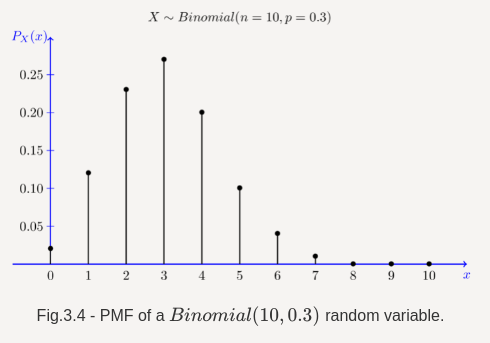
\includegraphics{Lecture 13 Notes e842fef9a3e0449fa78bac59b75dbc5c/Screenshot_from_2021-08-06_23-12-57.png}
  \caption{PMF of a binomial random variable}
  \end{figure}
\end{itemize}

\hypertarget{geometric-random-variables}{%
\subsubsection{3. Geometric Random
Variables}\label{geometric-random-variables}}

\begin{itemize}
\item
  Experiment: Toss a biased coin till a head is obtained. X is the
  position of the head.
\item
  \(P_X(k) = (1-p)^{k-1}p\)
\item
  \(E(X) = \displaystyle\sum_{i=0}^{n}i(1-p)^{i-1}p = 1/p\)
\item
  \(Var(X) =\) \(E(X^2) - (E(X))^2=E(X^2) -1/p^2\)

  \(E(X^2) = \displaystyle\sum_{k=1}^{\infty}k^2p(1-p)^{k-1}=(2-p)/p^2\)
\item
  \(\therefore Var(X) = (2-p-1)/p^2 = (1-p)/p^2\)

  \begin{figure}
  \centering
  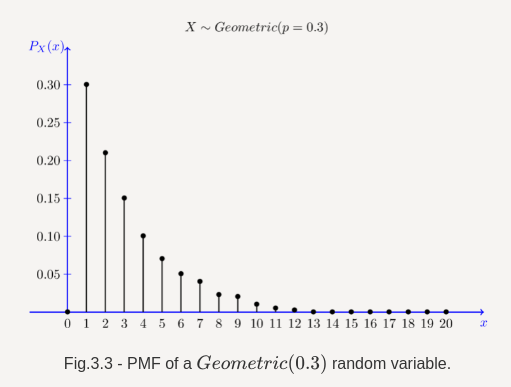
\includegraphics{Lecture 13 Notes e842fef9a3e0449fa78bac59b75dbc5c/Screenshot_from_2021-08-06_23-12-50.png}
  \caption{PMF of a geometric random variable}
  \end{figure}
\end{itemize}

\hypertarget{poisson-random-variables}{%
\subsubsection{4. Poisson Random
Variables}\label{poisson-random-variables}}

\begin{itemize}
\item
  Used to model rare events
\item
  \(P_X(k) = \lambda^ke^{-\lambda}/k!\)
\item
  \(E(X) = \lambda\)
\item
  \(Var(X) =\lambda\)

  \begin{figure}
  \centering
  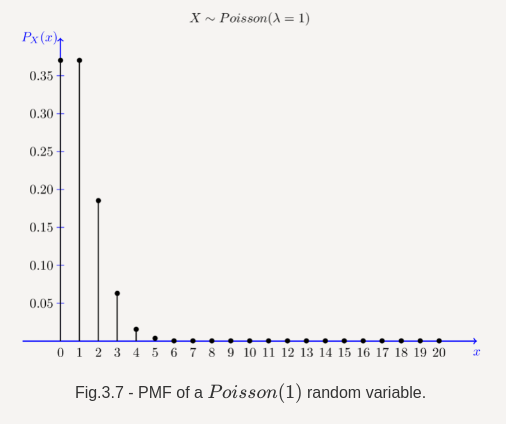
\includegraphics{Lecture 13 Notes e842fef9a3e0449fa78bac59b75dbc5c/Screenshot_from_2021-08-06_23-13-10.png}
  \caption{PMF of a poisson random variable}
  \end{figure}
\end{itemize}

\hypertarget{pascal-random-variables}{%
\subsubsection{5. Pascal Random
Variables}\label{pascal-random-variables}}

\begin{itemize}
\item
  This R.V can be understood as a generalisation of the geometric
  distribution.
\item
  Experiment: Biased coin with probability of heads being \(p\) tossed
  repeatedly until \(m\) heads are observed, \(m \in \mathcal{N}\).
\item
  As we can deduce from the above definition, a geometric variable is
  simply the case when \(m = 1\) for a Pascal random variable.
\item
  \(P_X(x) = \begin{cases}{{k-1}\choose{m-1}} p^m(1-p)^{k-m} & for \ k=m, m+1, m+2....\\0 & otherwise\end{cases}\)
\item
  \(E(X) = m/p\), can be derived by expressing it as the sum of multiple
  independent geometric random variables.
\item
  \(Var(X) = m\cdot (1-p)/p^2\)
\end{itemize}

\begin{figure}
\centering
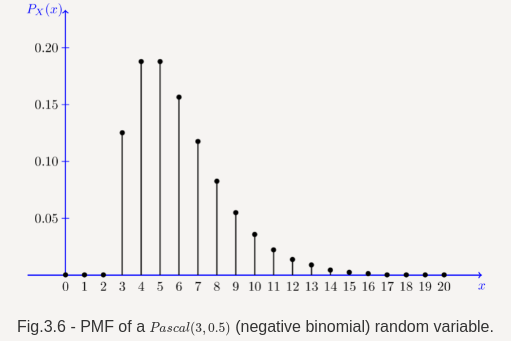
\includegraphics{../Screenshot from 2021-08-07 09-44-36.png}
\caption{PMF of a Pascal random variable}
\end{figure}

\begin{center}\rule{0.5\linewidth}{0.5pt}\end{center}

\hypertarget{examples-of-continuous-random-variables}{%
\subsection{Examples of Continuous Random
Variables}\label{examples-of-continuous-random-variables}}

\hypertarget{uniform-random-variables}{%
\subsubsection{1. Uniform Random
Variables}\label{uniform-random-variables}}

\begin{itemize}
\tightlist
\item
  \(f_X(x) = \begin{cases}1/(b-a) & for \ a\leq x\leq b\\0 & otherwise\end{cases}\)
\item
  \(E(X) = (a+b)/2\)
\item
  \(Var(X) = (b-a)^2/12\)
\end{itemize}

\begin{figure}
\centering
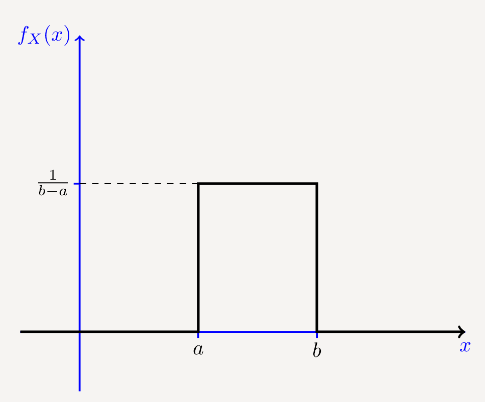
\includegraphics{Lecture 13 Notes e842fef9a3e0449fa78bac59b75dbc5c/Screenshot_from_2021-08-06_23-02-44.png}
\caption{PDF of a uniform random variable}
\end{figure}

\hypertarget{exponential-random-variables}{%
\subsubsection{2. Exponential Random
Variables}\label{exponential-random-variables}}

\begin{itemize}
\item
  Used to model completion time
\item
  \(f_X(x) = \begin{cases}\lambda e^{-\lambda x} & for x\geq 0\\0 & otherwise\end{cases}\)
\item
  \(E(X) = \displaystyle\int_{0}^{\infty}x\lambda e^{-\lambda x}dx=1/\lambda\)
\item
  \(Var(X) = 1/\lambda ^2\)

  \begin{figure}
  \centering
  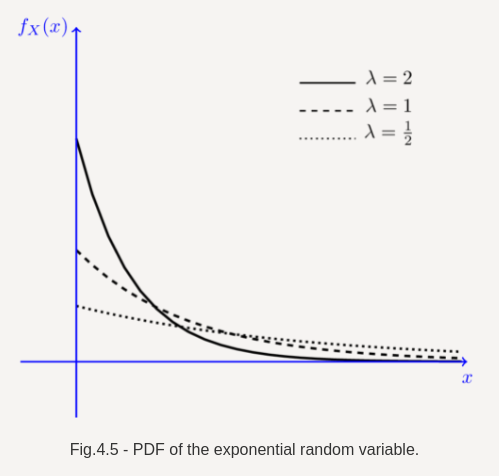
\includegraphics{Lecture 13 Notes e842fef9a3e0449fa78bac59b75dbc5c/Screenshot_from_2021-08-06_23-06-49.png}
  \caption{PDF of an exponential random variable}
  \end{figure}
\end{itemize}

\hypertarget{gaussian-random-variables}{%
\subsubsection{3. Gaussian Random
Variables}\label{gaussian-random-variables}}

\begin{itemize}
\item
  Used to model noise. It is a sum of many independent R.V.s
\item
  \(f_X(x) = \frac{1}{\sqrt{2\pi \sigma ^2}}e^\frac{-(x-\mu)^2}{2\sigma ^2}\)
\item
  \(E(X) = \mu\)
\item
  \(Var(X) = \sigma ^2\)

  \begin{figure}
  \centering
  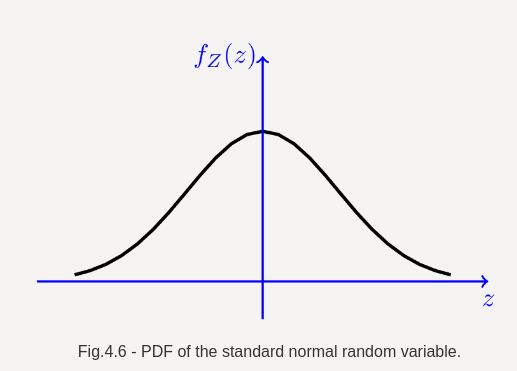
\includegraphics{Lecture 13 Notes e842fef9a3e0449fa78bac59b75dbc5c/Screenshot_from_2021-08-06_23-11-46.png}
  \caption{PDF of a standard normal random variable}
  \end{figure}
\end{itemize}

\begin{center}\rule{0.5\linewidth}{0.5pt}\end{center}
